\chapter{算法描述}
\section{单纯形法}
单纯形是$N$维中的$N+1$个顶点的凸包,是一个多胞体,譬如是直线上的一个线段,平面上的一个三角形,三维空间中的一个四面体等等,这些都是单纯形。

\begin{figure}[H]
	\centering
	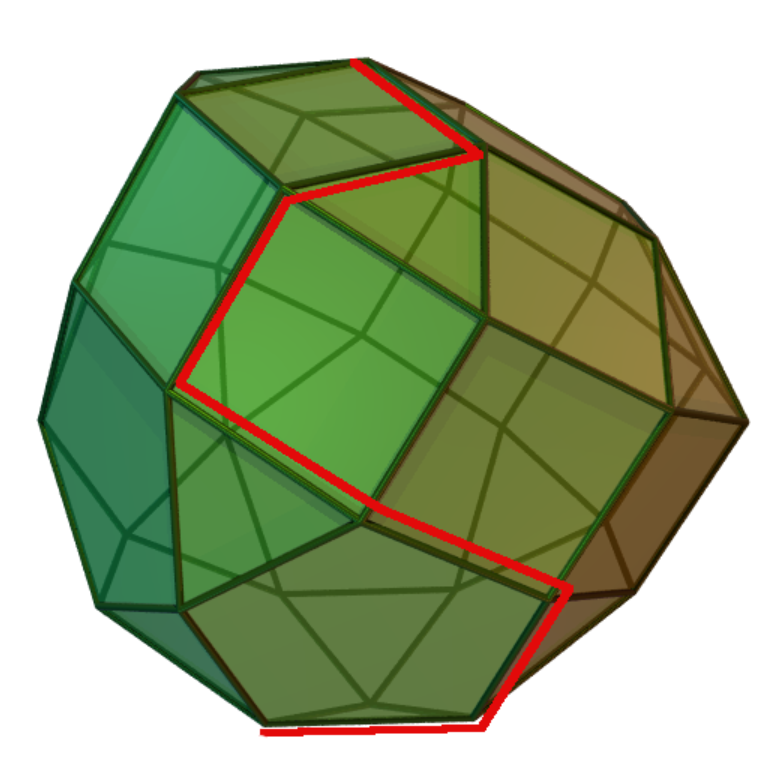
\includegraphics[scale=0.3]{contents/img/simplex.png}
	\caption{单纯形}
\end{figure}

\subsection{标准形式}
在使用单纯形法之前,我们需要将线性规划转换为以下标准形式:
$$
\begin{matrix}
\max&: & \sum\limits_{1 \le k \le n}c_{k}x_{k}\\
s.t.&: & Ax \le b \\
&  & x \ge 0
\end{matrix}
$$
所有其他形式的线性规划方程组都可以转化称这个标准形式:
\begin{itemize}
	\item[1] 目标函数不是极大化:只需要将$c_k$取为原来的相反数,就可以从极小化问题转化为极大化问题。
	\item[2] 约束条件中存在大于或等于约束:只需要将约束两边同乘$-1$。
	\item[3] 约束条件中存在等式:只需要将其转化为两个不等式,一个为大于等于,另一个为小于等于。
	\item[4] 有的变量约束为大于等于$R$:只需要做简单的仿射变换,用$x' = x - R$代替原来的变量即可。
	\item[5] 有的变量约束小于等于$0$:只需要将与该变量有关的所有系数取相反数即可。
	\item[6] 有的变量没有非负约束:加入新变量$x'$,并用$x - x'$替换原来的变量$x$。
\end{itemize}


通过以上总总,我们就可以将一个一般的线性规划转换为标准形式。

\subsection{松弛形式}
在使用单纯形法进行变换之前,我们需要先计算出一个可行解。我们可以通过将标准形式的线性规划转化为松弛形式,这样能够快速得到线性规划的初始可行解。只需要在原来$n$个变量,$m$个约束的线性规划中,加入$m$个新变量,就可以将原来的不等式化为等式:
$$
\forall j \in \{1, 2, \dots, m\}, \\
\sum\limits_{1 \le k \le n} a_{j, k}x_{k} + x_{n+j} = b_{j}, \\
x_{n+j} \ge 0
$$
我们可以首先通过新加入的变量快速得到一组初始可行解:
$$
x_{n+j} = b_{j} - \sum\limits_{1 \le k \le n} a_{j,k}x_{k}
$$
我们现在称$x_{1}, x_{2}, \dots, x_{n}$这些变量为\textbf{非基变量},而称$x_{n+1}, x_{n+2}, \dots, x_{n+m}$这些变量为\textbf{基变量}。非基变量能够由基变量唯一确定,也就是课上老师所说的\textbf{典则形式}。

我们通过两阶段法求得原标准形式的初始可行解:
\begin{itemize}
	\item[1] 第一阶段的目标函数为$\min: \sum\limits_{n+1 \le k \le n+m}x_{n+k}$, 如果得到该目标函数值为$0$,则通过转轴变换将基变量全部转换为原来的变量。如果目标函数值非$0$,则表明原规划问题无解。
	\item[2] 第一阶段结束以后,以第一阶段得到的可行解进行求解原始问题。
\end{itemize}

\textbf{单纯形表}则是将松弛形式(或者标准形式)的规划问题中的系数放入一个增广矩阵中,通过矩阵变换求得最终的最优解和最优值。

\subsection{转轴变换}
转轴变换是单纯形法中的核心操作,作用就是将一个基变量与一个非基变量进行互换。从几何的理解上就是从单纯形的一个极点走向另一个极点。设变量$x_{n+d}$是基变量,变量$x_{e}$是非基变量,那么转轴操作\textbf{pivot(d, e)}以后,$x_{n+d}$将变为非基变量,相应的$x_{e}$变为基变量。将这些转化为用数学符号描述则如下:
$$
\begin{matrix}
\text{起初}& : & x_{n+d} = b_{d} - \sum\limits_{k \in N}a_{d, k}x_{k} \\
\text{移项}& : & a_{d, e}x_{e} = b_{d} - \sum\limits_{k \in N \and k \ne e} a_{d, k}x_{k} - x_{n+d} \\
\text{若}a_{d, e} \ne 0 & : & x_{e} = \dfrac{b_{d}}{a_{d, e}} - \sum\limits_{k \in N \and k \ne e}\dfrac{a_{d, k}}{a_{d, e}}x_{k} - \dfrac{1}{a_{d, e}}x_{n+d}
\end{matrix}
$$
将这个式子代入其他的约束等式以及目标函数中,就实现了$x_{n+d}$和$x_{e}$的基变量与非基变量的转换。

这在增广矩阵中的操作则对应为第$i$行的基变量变为第$j$个变量,然后利用消元法将其他行中第$j$列的系数消去。我们称这个操作为转轴变换。

\subsection{最优化过程}
而我们挑选哪一个非基变量与基变量进行转轴变换则是最优化过程了,这个过程如下:
\begin{itemize}
\item 得到原规划问题的初始可行解(两阶段法)
\item 任取一个非基变量$x_{e}$,使得$c_{e} > 0$
\item 考虑基变量$x_{d}$,$\min\limits_{a_{d, e} > 0} \dfrac{b_{d}}{a_{d, e}}$ 
\item 交换$x_{e}和x_{d}$, 即转轴变换\textbf{pivot(d, e)} 
\item 如果所有的非基变量的系数都是小于等于$0$时,我们已经得到最优解了。将基变量及其增广列对应值作为输出即可。
   		  如果只剩$c{e} > 0$且$\forall i \in \{1, 2, \dots, m\}, a_{d, e} \le 0$ 则原规划问题没有有限最有解,目标函数值为正无穷。	
\end{itemize}


\subsection{Bland法则}
而我们选取非基变量入基的时候,不能够每次都选择检验数最大的入基,这样会导致单纯形法退化,进入搜索循环的bug。根据\textbf{Bland法则},我们可以每次选择下标最小的非基变量入基,就可以避免单纯形法退化。

\section{分枝定界法}
分枝定界法不只是解决整数规划的一种方法,它其实可以认为是一种组合优化问题以及数学优化算法设计的范式。 分枝定界法由通过状态空间搜索的候选解决方案的系统枚举组成:候选解决方案集被认为是在根处形成具有全集的根树。 该算法探索此树的分支,它代表解决方案集的子集。 在枚举分支的候选解之前,针对最优解的\textbf{上下估计边界检查分支},并且如果它不能产生比迄今为止由算法找到的最佳解决方案更好的解,则丢弃该分支(\textbf{称为剪枝})。

在整数规划问题中,我们先将原问题放松成线性规划问题,解这个线性规划,就得到了整数规划最优解的上界。这是因为减少了约束,得到的目标函数值自然更大,所以是上界。然后我们检查最优解,如果最优解中有非整数变量,记为$x_{i}$, $N < x_{i} < N+1$,这时候就会有两种可能:$x_{i} \le N$或者$x_{i} \ge N+1$。这时候我们分枝,一枝增加约束$x_{i} \le N$,另一枝增加约束$x_{i} \ge N+1$。然后递归进行搜索。如果中间过程得到的线性规划最优解也是整数规划最优解,就记其为下界。如果某一枝的上界比下界还小,则将这一枝剪去,称为剪枝,这一枝称为死枝。直到最后找到最优解。中间过程中需要反复降为线性规划以单纯形法进行求解。

这里我们分枝定界法是需要维护两个界的,一个是上界,一个是下界:
\begin{itemize}
\item 上界初始化为没有增加约束的原问题的线性规划最优解
  \begin{itemize}
	  \item 更新则在于从一个节点分成两个节点后,取两个节点中线性规划的最优解的最大值。
  \end{itemize}
\item 下界初始化为负无穷
  \begin{itemize}
	  \item 更新则在于每次求解出一个线性规划也正好为整数规划且比已知的下界大时,更新下界。
  \end{itemize}
\item 如果计算得到的线性规划最优解比已知的下界小,则进行剪枝。
\item 如此计算,上界会不断减小,下界会不断提高,直到上界等于下界。
\end{itemize}

\begin{figure}[H]
	\centering
	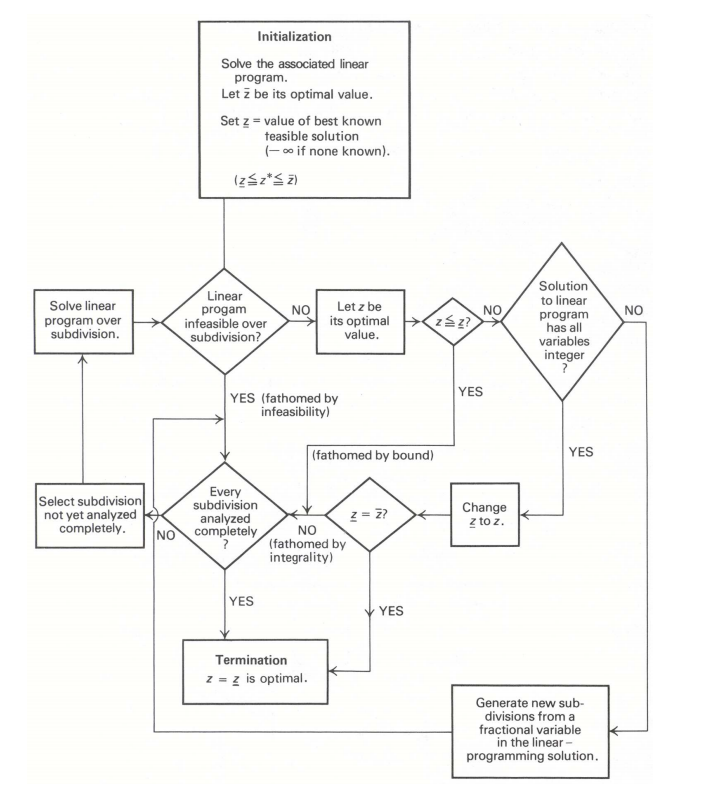
\includegraphics[width=\textwidth,height=\textheight,keepaspectratio]{contents/img/BB.png}
	\caption{分枝定界算法流程图}
\end{figure}

